\documentclass[12pt,a4paper]{article}

% ─── Page Layout ───────────────────────────────────────────────────────────────
\usepackage[a4paper, margin=0.8in, headheight=14pt]{geometry}

% ─── Fonts (XeLaTeX) ───────────────────────────────────────────────────────────
\usepackage{fontspec}
\usepackage{unicode-math}
\setmainfont{TeX Gyre Pagella}
\setmonofont[Scale=0.88]{TeX Gyre Cursor}
\setmathfont{Latin Modern Math}

% ─── Packages ──────────────────────────────────────────────────────────────────
\usepackage{xcolor}
\usepackage{colortbl}
\usepackage{titlesec}
\usepackage{enumitem}
\usepackage{tabularx}
\usepackage{booktabs}
\usepackage{array}
\usepackage{amsmath}
\usepackage{tikz}
\usetikzlibrary{shapes.geometric, arrows.meta, positioning, calc, fit, decorations.pathreplacing}
\usepackage{tcolorbox}
\tcbuselibrary{skins, breakable}
\usepackage{hyperref}
\usepackage{fancyhdr}
\usepackage{graphicx}
\usepackage{microtype}
\hyphenpenalty=10000
\exhyphenpenalty=10000
\sloppy
\usepackage{caption}
\usepackage{setspace}
\usepackage{multirow}
\usepackage{tocloft}

% ─── Q&A helper ────────────────────────────────────────────────────────────────
\newcommand{\Q}[1]{\textbf{#1}\par\noindent\ignorespaces}

% ─── Colour Palette ────────────────────────────────────────────────────────────
\definecolor{myred}{RGB}{196,30,58}
\definecolor{mydark}{RGB}{30,30,50}
\definecolor{mygreen}{RGB}{14,120,80}
\definecolor{myteal}{RGB}{0,130,140}
\definecolor{myamber}{RGB}{180,100,0}
\definecolor{mypurple}{RGB}{100,30,160}
\definecolor{mygray}{RGB}{246,247,249}
\definecolor{mgframe}{RGB}{180,185,200}
\definecolor{watermark}{RGB}{145,150,170}
\definecolor{hdrred}{RGB}{250,232,235}
\definecolor{hdrgreen}{RGB}{220,244,233}
\definecolor{hdrteal}{RGB}{220,242,244}
\definecolor{hdramber}{RGB}{253,242,215}
\definecolor{hdrpurple}{RGB}{238,228,255}
\definecolor{hdrgray}{RGB}{238,240,245}
\definecolor{rowalt}{RGB}{250,251,253}

% ─── Section Formatting ────────────────────────────────────────────────────────
\titleformat{\section}
  {\large\bfseries\color{myred}}{\thesection.}{0.5em}{}
  [\vspace{1pt}{\color{myred}\rule{\linewidth}{0.8pt}}]
\titleformat{\subsection}
  {\normalsize\bfseries\color{myteal}}{\thesubsection}{0.5em}{}
\titlespacing*{\section}{0pt}{18pt}{7pt}
\titlespacing*{\subsection}{0pt}{11pt}{4pt}

% ─── Paragraph ─────────────────────────────────────────────────────────────────
\setlength{\parindent}{0pt}
\setlength{\parskip}{4pt}

% ─── TOC Styling ───────────────────────────────────────────────────────────────
\renewcommand{\cfttoctitlefont}{\large\bfseries\color{myred}}
\renewcommand{\cftaftertoctitle}{\par\noindent{\color{myred}\rule{\linewidth}{0.8pt}}}
\setlength{\cftbeforetoctitleskip}{0pt}
\setlength{\cftaftertoctitleskip}{6pt}
\renewcommand{\cftsecfont}{\normalsize\bfseries\color{mydark}}
\renewcommand{\cftsecpagefont}{\normalsize\bfseries\color{mydark}}
\renewcommand{\cftsecleader}{\cftdotfill{\cftdotsep}}
\setlength{\cftbeforesecskip}{7pt}
\renewcommand{\cftsubsecfont}{\small\color{mydark}}
\renewcommand{\cftsubsecpagefont}{\small\color{mydark}}
\setlength{\cftbeforesubsecskip}{3pt}
\setlength{\cftsubsecindent}{1.4em}

% ─── Table helpers ─────────────────────────────────────────────────────────────
\renewcommand{\arraystretch}{1.45}
\setlength{\tabcolsep}{6pt}
\arrayrulecolor{mydark}
\newcolumntype{B}[1]{>{\small\bfseries\raggedright\arraybackslash}m{#1}}
\newcolumntype{Y}{>{\small\raggedright\arraybackslash}X}
\renewcommand{\tabularxcolumn}[1]{m{#1}}

% ─── Header / Footer ───────────────────────────────────────────────────────────
\pagestyle{fancy}
\fancyhf{}
\fancyhead[L]{\small\color{myred}\textbf{EC502}\;\color{mydark}--- Computer Architecture}
\fancyhead[R]{\small\color{myteal}\textbf{Module 5 Notes}}
\fancyfoot[C]{\small\color{mydark}\thepage}
\fancyfoot[R]{\small\color{watermark}\textit{\copyright\ Biraj}}
\renewcommand{\headrulewidth}{0.5pt}
\renewcommand{\footrulewidth}{0.3pt}

% ─── Hyperref ──────────────────────────────────────────────────────────────────
\hypersetup{
  colorlinks=true, linkcolor=myteal, urlcolor=myteal,
  pdfauthor={Biraj Sarkar},
  pdftitle={EC502 --- Module 5 Notes}
}

% ─── tcolorbox styles ──────────────────────────────────────────────────────────
\tcbset{
  tikzbox/.style={
    colback=mygray, colframe=mgframe, boxrule=0.6pt, arc=4pt,
    left=8pt, right=8pt, top=6pt, bottom=6pt,
    colbacktitle=mgframe, coltitle=mydark,
    fonttitle=\small\bfseries
  },
  defbox/.style={
    colback=hdrgreen, colframe=mygreen, boxrule=0.8pt, arc=4pt,
    left=9pt, right=9pt, top=6pt, bottom=6pt,
    colbacktitle=mygreen, coltitle=white,
    fonttitle=\small\bfseries
  },
  formulabox/.style={
    colback=hdrteal, colframe=myteal, boxrule=0.8pt, arc=4pt,
    left=9pt, right=9pt, top=7pt, bottom=7pt,
    colbacktitle=myteal, coltitle=white,
    fonttitle=\small\bfseries
  },
  examplebox/.style={
    colback=hdramber, colframe=myamber, boxrule=0.8pt, arc=4pt,
    left=9pt, right=9pt, top=6pt, bottom=6pt,
    colbacktitle=myamber, coltitle=white,
    fonttitle=\small\bfseries
  },
  masonbox/.style={
    colback=hdrpurple, colframe=mypurple, boxrule=0.8pt, arc=4pt,
    left=9pt, right=9pt, top=6pt, bottom=6pt,
    colbacktitle=mypurple, coltitle=white,
    fonttitle=\small\bfseries
  },
  exambox/.style={
    colback=hdrpurple, colframe=mypurple, boxrule=1pt, arc=5pt,
    left=10pt, right=10pt, top=8pt, bottom=8pt,
    colbacktitle=mypurple, coltitle=white,
    fonttitle=\bfseries,
    breakable, title after break={\textbf{Frequently Asked / Viva Questions (contd.)}}}
}
% Make all boxes breakable across pages
\tcbset{breakable}

% ─── TikZ styles ───────────────────────────────────────────────────────────────
\tikzset{
  block/.style={rectangle, draw=myteal, fill=hdrteal,
    text width=2.4cm, align=center, minimum height=0.95cm,
    font=\small, rounded corners=3pt, line width=0.7pt},
  redblock/.style={rectangle, draw=myred, fill=hdrred,
    text width=2.4cm, align=center, minimum height=0.95cm,
    font=\small, rounded corners=3pt, line width=0.7pt},
  netnode/.style={rectangle, draw=myteal, fill=hdrteal,
    text width=1.5cm, align=center, minimum height=0.8cm,
    font=\small, rounded corners=3pt, line width=0.7pt},
  sumjunc/.style={circle, draw=myamber, fill=hdramber,
    minimum size=0.62cm, font=\small, line width=0.8pt},
  snode/.style={circle, draw=mypurple, fill=hdrpurple,
    minimum size=0.55cm, font=\footnotesize, line width=0.7pt},
  arrow/.style={-Stealth, thick, color=mydark},
  redarrow/.style={-Stealth, thick, color=myred},
  line/.style={thick, color=mydark}
}

% ═══════════════════════════════════════════════════════════════════════════════
\begin{document}
% ═══════════════════════════════════════════════════════════════════════════════

\begin{center}
  {\LARGE\bfseries\color{myred} EC502 --- Computer Architecture}\\[5pt]
  {\normalsize\color{mydark} Semester V \quad$\bullet$\quad 3L:0T:0P \quad$\bullet$\quad 3 Credits}\\[3pt]
  {\normalsize\color{myteal}\textbf{Module 5 Exam Notes: Memory Organisation and Virtual Memory}}\\[3pt]
  {\small\color{mydark} CGEC \;$|$\; B.Tech ECE (2023--27) \;$|$\; \textit{Biraj Sarkar}}
\end{center}
\vspace{2pt}
\noindent{\color{myred}\rule{\linewidth}{1.5pt}}
\vspace{2pt}

\hypersetup{linkcolor=mydark}
\tableofcontents
\hypersetup{linkcolor=myteal}
\newpage

\section{Memory Organisation and Virtual Memory}
\begin{tcolorbox}[defbox,title={Memory hierarchy}]
A memory hierarchy places small fast storage near the processor and larger slower storage farther away. Recent reuse (temporal locality) and access to nearby addresses (spatial locality) help a small upper level serve many references.
\end{tcolorbox}
\begin{tcolorbox}[tikzbox,title={Hierarchy and the direction of the trade-off},unbreakable]
\centering
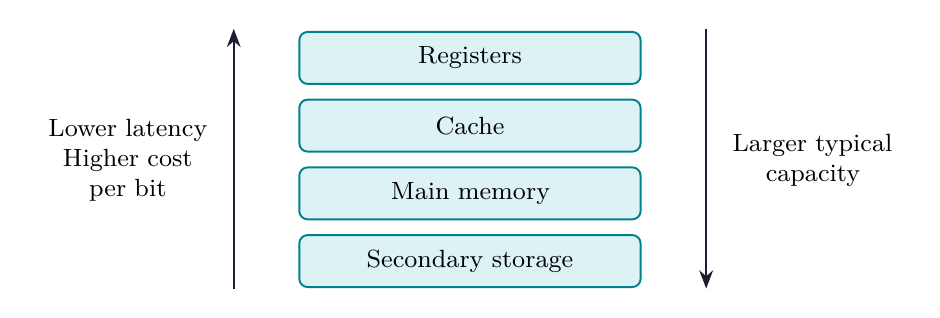
\begin{tikzpicture}[font=\small]
\foreach \y/\name in {0/Registers,-.86/Cache,-1.72/Main memory,-2.58/Secondary storage}{
 \node[block,text width=4.1cm,minimum height=.66cm] at (0,\y) {\name};
}
\draw[arrow] (-3,-2.93)--(-3,.37);
\node[align=center,text width=2.3cm] at (-4.35,-1.3) {Lower latency\\Higher cost per bit};
\draw[arrow] (3,.37)--(3,-2.93);
\node[align=center,text width=2.3cm] at (4.35,-1.3) {Larger typical\\capacity};
\end{tikzpicture}
\end{tcolorbox}

\subsection{Device characteristics and chip organisation}
\begin{itemize}[leftmargin=*,itemsep=3pt]
\item \textbf{Capacity.} A memory of $2^a$ words, each $w$ bits wide, stores $2^aw$ bits. It needs $a$ logical word-address bits. Physical pins may multiplex row and column addresses.
\item \textbf{Latency and cycle time.} Access time is the delay from request to usable data. Cycle time is the minimum interval between suitable successive operations. Transfer bandwidth is bits or bytes transferred per unit time. Burst access can have a high first-word latency but good bandwidth.
\item \textbf{Volatility and endurance.} Volatile devices lose data without power. Nonvolatile devices retain it. Some nonvolatile devices have erase-block constraints and finite program/erase endurance.
\item \textbf{Control and banks.} Chip select enables one chip group. Read/write or output-enable signals control the transfer. With low-order interleaving, word $A$ goes to bank $A\bmod B$ and row $\lfloor A/B\rfloor$ for $B$ banks. Consecutive accesses can overlap if controllers and banks permit.
\end{itemize}
\begin{tcolorbox}[examplebox,title={Build a wider and deeper memory}]
Build $16\mathrm{K}\times16$ from $4\mathrm{K}\times8$ chips, with $\mathrm K=1024$.
\begin{enumerate}[leftmargin=*,itemsep=2pt]
\item Width: two chips in parallel share the address and control signals. One supplies each byte.
\item Depth: four banks of two chips give $16\mathrm K$ word addresses, using eight chips total.
\item Decode: 12 low word-address bits go to every chip. Two high word-address bits select one bank. The total data width is 16 bits. In a byte-addressed host, one additional low address bit selects the byte within a word.
\end{enumerate}
\end{tcolorbox}

\subsection{RAM, ROM and memory technologies}
Random-access memory (RAM) supports read/write access by address. Read-only memory (ROM) families retain data without power and differ in how they can be programmed.
\par\vspace{6pt}\noindent
\begin{tabularx}{\linewidth}{|B{3cm}|Y|Y|}\hline
Device & Storage and operation & Common role \\ \hline
Static RAM (SRAM) & A typical CMOS cell uses six transistors in a latch and access path. State persists while powered without refresh. & Fast but less dense. Common in caches and small on-chip memories. \\ \hline
Dynamic RAM (DRAM) & A typical cell uses one transistor and one capacitor. Charge leaks, so refresh is required. Sense amplifiers restore data after reading. Row activation opens a row buffer. & Dense, volatile main memory. Row hits can be faster than opening a different row. \\ \hline
Synchronous DRAM (SDRAM) & DRAM commands and transfers are coordinated by a clocked interface. A burst can transfer several words per command. Double-data-rate (DDR) families transfer data on both clock edges. & Main memory. Synchronous timing describes the interface, not a different basic bit cell. \\ \hline
Mask ROM / PROM & Mask ROM is fixed in manufacture. Programmable ROM (PROM) can be programmed once afterwards. & Fixed firmware or tables. \\ \hline
EPROM / EEPROM & Erasable PROM (EPROM) typically uses ultraviolet erase. Electrically erasable PROM (EEPROM) can be erased and programmed electrically. & Nonvolatile programming and configuration. \\ \hline
Flash & A dense electrically erasable memory typically erased in blocks, with different read, program and erase granularities. & Firmware storage, cards and solid-state drives. \\ \hline
\end{tabularx}

\subsection{Read and write a six-transistor SRAM cell}
Two cross-coupled inverters store complementary nodes $Q$ and $\overline Q$. Two access transistors connect them to complementary bit lines BL and $\overline{\mathrm{BL}}$ when the word line is asserted.
\begin{enumerate}[leftmargin=*,itemsep=3pt]
\item \textbf{Hold:} with the word line low, the cell is isolated from the bit lines and the feedback loop retains the state while power is supplied.
\item \textbf{Read:} precharge both bit lines, then raise the word line. The side storing zero discharges its bit line slightly. A sense amplifier detects the difference. Cell sizing prevents the read from flipping the latch.
\item \textbf{Write:} drive complementary bit-line values for the desired state and raise the word line. The write drivers overcome the latch's feedback. Lower the word line after the new state has settled.
\end{enumerate}

\section{Cache and Associative Memories}
\begin{tcolorbox}[defbox,title={Cache line, hit and miss}]
A cache keeps copies of recently used memory blocks in fixed-size lines. A hit finds a valid matching tag. A miss fetches or otherwise services data at a lower level. Block offset selects a byte inside a line.
\end{tcolorbox}
\subsection{Mapping and address fields}
Let byte addresses have $m$ bits, block size $B=2^b$ bytes, data capacity $C$, and associativity $W$ ways. Then the number of sets is $S=C/(WB)$. For $S=2^s$, split the address into $(m-b-s)$ tag bits, $s$ index bits and $b$ offset bits. Divide address by $B$ for the block number. Set is block number modulo $S$.
\par\vspace{6pt}\noindent
\begin{tabularx}{\linewidth}{|B{3.2cm}|Y|Y|}\hline
Mapping & Placement and lookup & Main trade-off \\ \hline
Direct mapped & One line per set. One index-selected tag comparison. & Simple and fast. Blocks with the same index can repeatedly displace each other. \\ \hline
Set associative & $W$ choices in the indexed set. Compare its $W$ tags and select a hit way. & Fewer conflict misses, with more comparators and replacement state. \\ \hline
Fully associative & One set. The block can occupy any line and there are no index bits. & Flexible placement. Parallel lookup of many tags can be expensive. \\ \hline
\end{tabularx}

\begin{tcolorbox}[examplebox,title={Decode an address in a four-way cache}]
A 32-bit byte address is used with a $32\,\mathrm{KiB}$ data cache, four ways and 64-byte lines. The cache has $32768/(4\cdot64)=128$ sets. Thus offset, index and tag lengths are 6, 7 and 19 bits respectively. For \texttt{0x12345678}, the offset is \texttt{0x38}, index \texttt{0x59}, and tag \texttt{0x91A2}. Look for this tag in the four lines of set 89. A matching tag with valid bit clear is still a miss.
There are $128(4)=512$ lines. Tag bits alone require $512(19)=9728$ bits. A valid and a dirty bit per line would add $1024$ bits. Replacement state, coherence metadata and error protection are separate costs.
\end{tcolorbox}

\subsection{Replacement, write policy and access time}
\begin{itemize}[leftmargin=*,itemsep=3pt]
\item \textbf{Replacement.} Use an empty way first. If the set is full, policies such as least recently used (LRU), FIFO or random select a victim. An evicted dirty line must be written back.
\item \textbf{Miss classification.} Compulsory misses occur on the first touch. Capacity misses arise when the working set exceeds capacity even with flexible placement. Conflict misses arise from placement restrictions. Coherence traffic can add misses in multicore systems.
\item \textbf{Write hit.} Write-through updates the lower level on the write, often through a buffer. Write-back updates only the cache and marks the line dirty until eviction or a required flush.
\item \textbf{Write miss.} Write-allocate fills and updates a line. No-write-allocate sends the write downstream without filling that line. These choices are separate from the write-hit policy.
\item \textbf{Reduce the miss penalty.} A fast lower-level cache can service misses without waiting for main memory. Critical-word-first fetches the requested word first. Early restart lets execution resume as soon as that word arrives. Write buffers can decouple a dirty eviction or a write-through update from the processor, subject to ordering and buffer capacity.
\end{itemize}
\begin{tcolorbox}[examplebox,title={Trace LRU and calculate average memory access time}]
For a two-way four-set cache, access block numbers $0,4,0,8,4$ from an empty state. Every reference uses set 0. Outcomes are miss, miss, hit, miss, miss. Block 4 is evicted on the fourth access because block 0 was more recently used. On the fifth access block 0 is the older remaining victim.

Average memory access time (AMAT) is hit time plus miss rate times additional miss penalty. For L1 time $1\,\mathrm{ns}$, L1 miss rate $0.05$, L2 time $10\,\mathrm{ns}$, local L2 miss rate $0.20$, and added main-memory penalty $80\,\mathrm{ns}$:
\[
 \mathrm{AMAT}=1+0.05(10+0.20\cdot80)=2.3\,\mathrm{ns}.
\]
The overall L2 miss fraction relative to all CPU accesses is $0.05(0.20)=0.01$.
\end{tcolorbox}
\begin{tcolorbox}[examplebox,title={Weight read and write timings separately}]
Assume a serial cache lookup of $4\,\mathrm{ns}$, added memory time of $60\,\mathrm{ns}$, read hit rate $0.90$, and no write buffer. Reads are $75\%$ of references. In this model a write-through store always needs one added memory access, including on a hit. Assume a write miss bypasses allocation.
\[
\begin{aligned}
T_{\rm read}&=4+(1-0.90)60=10\,\mathrm{ns},\\
T_{\rm write}&=4+60=64\,\mathrm{ns},\\
T_{\rm avg}&=0.75(10)+0.25(64)=23.5\,\mathrm{ns}.
\end{aligned}
\]
State the assumed write policy, hit cost and whether memory timing overlaps the cache lookup before averaging.
\end{tcolorbox}

\subsection{Associative memory and tag comparison}
Content-addressable memory (CAM) looks up data \emph{by contents} and returns matches rather than reading by a supplied address. A CAM row compares its enabled bits against a search key in parallel. A match line reports full-row equality and a priority encoder can select one result if allowed. A mask can ignore chosen bits. Parallel comparators make lookup fast but cost silicon area and energy. Small fully associative tables, including some translation lookaside buffers, use this principle.

\section{Memory Management and Virtual Addresses}
\begin{tcolorbox}[defbox,title={Virtual memory and address translation}]
Virtual memory gives a process a protected virtual address space. A memory management unit (MMU) translates supported virtual addresses to physical addresses. The operating system maintains mappings and may load or reclaim pages as needed.
\end{tcolorbox}

\subsection{Base, limit, segmentation and paging}
\begin{itemize}[leftmargin=*,itemsep=3pt]
\item \textbf{Base and limit.} Check $0\le v<\mathrm{limit}$ before calculating physical address $\mathrm{base}+v$. This supports relocation and protection but needs a contiguous physical region.
\item \textbf{Segmentation.} A segment selector identifies a base, length and permissions. A segment offset is checked against its limit. Variable segment sizes can cause external fragmentation.
\item \textbf{Paging.} With $2^p$-byte pages, split virtual address into virtual page number (VPN) and $p$ offset bits. A page table entry (PTE) supplies a physical frame and status such as valid/present, permissions, accessed and dirty. Copy the offset unchanged into the physical address. Fixed-size frames remove external fragmentation for page allocation, but the last page may have unused space.
\item \textbf{Multilevel table.} Split the VPN across levels. Intermediate entries point to smaller page tables and the final entry maps to a frame. Sparse spaces can leave entire unused lower tables unallocated.
\end{itemize}
\begin{tcolorbox}[tikzbox,title={Virtual page translation and unchanged offset},unbreakable]
\centering
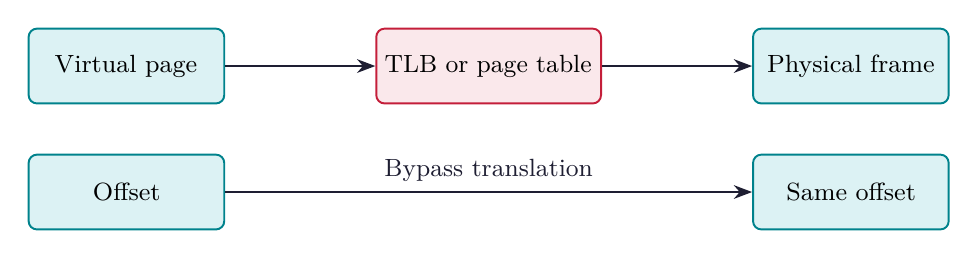
\begin{tikzpicture}[font=\small]
\node[block,text width=2.25cm] (v) at (0,0) {Virtual page};
\node[redblock,text width=2.62cm] (t) at (4.6,0) {TLB or page table};
\node[block,text width=2.25cm] (p) at (9.2,0) {Physical frame};
\node[block,text width=2.25cm] (o) at (0,-1.6) {Offset};
\node[block,text width=2.25cm] (z) at (9.2,-1.6) {Same offset};
\draw[arrow] (v.east)--(t.west);
\draw[arrow] (t.east)--(p.west);
\draw[arrow] (o.east)--(z.west) node[midway,above] {Bypass translation};
\end{tikzpicture}
\end{tcolorbox}

\subsection{TLB miss versus page fault}
\begin{enumerate}[leftmargin=*,itemsep=3pt]
\item \textbf{TLB hit.} The translation lookaside buffer (TLB) caches recent translations and access permissions. Check protection and form the physical address.
\item \textbf{TLB miss.} Walk the page table in hardware or software. If a usable entry exists, fill the TLB and continue. Main-memory residency is independent of whether the translation was cached.
\item \textbf{Page fault.} Trap to the operating system for a missing page, disallowed access or other fault condition. For a valid demand-page miss, obtain a frame, write a dirty victim if necessary, load or initialise the page, update mappings and restart the instruction. An illegal access may instead terminate the operation.
\item \textbf{Replacement and working set.} FIFO, LRU approximations and clock policies choose a victim. A working set is the group of actively used pages. If too few frames hold it, repeated faults can cause thrashing. Page replacement operates on main-memory frames, not CPU cache lines.
\end{enumerate}
\begin{tcolorbox}[examplebox,title={Translate an address and compute TLB timing}]
With $4\,\mathrm{KiB}$ pages, \texttt{0x12345} splits into VPN \texttt{0x12} and offset \texttt{0x345}. If that VPN maps to frame \texttt{0x2A}, the physical address is \texttt{0x2A345}.

Assume a serial 1 ns TLB lookup, 80 ns memory access, a one-access page-table walk, 98\% TLB hits and no page faults. A hit takes $81\,\mathrm{ns}$ and a miss $161\,\mathrm{ns}$. Mean access time is $0.98(81)+0.02(161)=82.6\,\mathrm{ns}$. Add a separate weighted fault-service cost only if the model specifies a page-fault probability.
\end{tcolorbox}

\begin{tcolorbox}[examplebox,title={Size a set-associative TLB tag}]
With 36-bit virtual byte addresses and $8\,\mathrm{KiB}$ pages, the offset is 13 bits and the VPN has 23 bits. A 128-entry four-way TLB has 32 sets, so the index takes five VPN bits. The virtual tag is $23-5=18$ bits, excluding any address-space identifier or page-size field. The physical frame number is stored data and does not contribute to this virtual tag length.
\end{tcolorbox}

\newpage
\begin{center}
  {\large\bfseries\color{myred} Quick Revision --- Module 5}\\[3pt]
  {\small\color{mydark} Memory Organisation and Virtual Memory $|$ EC502}
\end{center}
\noindent{\color{myred}\rule{\linewidth}{1.2pt}}
\begin{tcolorbox}[formulabox,title={Key Formulas at a Glance}]
\renewcommand{\arraystretch}{1.35}
\begin{tabularx}{\linewidth}{B{5.0cm}Y}
Chip capacity & $2^a$ words of $w$ bits equals $2^aw$ bits \\[3pt]
Cache sets & $S=C/(WB)$ for capacity $C$, block size $B$, and $W$ ways \\[3pt]
Cache fields & Offset $\log_2B$, index $\log_2 S$, remaining tag bits \\[3pt]
AMAT & Hit time plus miss rate times additional penalty \\[3pt]
Paging & Physical frame number concatenated with unchanged page offset \\[3pt]
\end{tabularx}
\end{tcolorbox}
\begin{tcolorbox}[defbox,title={One-Line Definitions}]
\textbf{Locality.} Tendency to reuse recent addresses or access nearby addresses.\par
\textbf{Associative memory.} Memory that finds entries matching a content key.\par
\textbf{TLB.} Fast cache of recent virtual-to-physical translations and permissions.\par
\end{tcolorbox}
\begin{tcolorbox}[exambox,title={Frequently Asked / Viva Questions}]
\begin{enumerate}[topsep=0pt, label=\textbf{Q\arabic*.}, itemsep=5pt]
\item \Q{Why does DRAM need refresh?}
Stored capacitor charge leaks.
\item \Q{Why is SRAM commonly used in processor caches?}
It has low latency and does not require refresh while powered.
\item \Q{What is the role of a cache tag?}
Identify the particular memory block occupying a line.
\item \Q{Can a direct-mapped cache choose among victims?}
No, each block has exactly one possible line.
\item \Q{What does a dirty bit say?}
The upper copy was modified and may need write-back.
\item \Q{Which miss remains when capacity and placement are unlimited?}
A first access still causes a compulsory miss.
\item \Q{Which cache mapping has zero index bits?}
Fully associative mapping has one set.
\item \Q{Does a TLB miss imply a page fault?}
No. A table walk may find a valid resident mapping.
\item \Q{What is unchanged by paging translation?}
The offset within the page or frame.
\item \Q{Why can thrashing reduce useful progress?}
Repeated page faults dominate execution time.
\end{enumerate}
\end{tcolorbox}
\begin{tcolorbox}[tikzbox,title={Summary comparison}]
\begin{tabularx}{\linewidth}{|B{4cm}|Y|}\hline
\textbf{Case} & \textbf{What to use} \\ \hline
SRAM / DRAM & Latch without refresh / capacitor storage with refresh. \\ \hline
Cache / virtual memory & Speed up block reuse / translate and protect address spaces. \\ \hline
TLB miss / page fault & Translation lookup refill / operating-system trap. \\ \hline
\end{tabularx}
\end{tcolorbox}
\end{document}
